\documentclass[aspectratio=169]{beamer}
% language and font set up
\usepackage[utf8]{inputenc}
\usepackage{amsmath}
\usepackage{amsfonts}
% additonal packages
\usepackage{graphicx}
\usepackage{color}
\usepackage{listings}
\usepackage{hyperref}
% design
\usetheme{Berlin}
% \usecolortheme{beaver}
% informations
\title{Gödel's Incompletness Theorems}
\author{Lukas Wais}
\institute{Special Topics Course 326.901}
\date{\today}

\begin{document}
% title frame
\frame{\titlepage}
% table of content
\begin{frame}[allowframebreaks]
	\frametitle{Table of Contents}
	\tableofcontents
\end{frame}
% introduction
\section{Introduction}
\subsection{Who was Kurt Gödel}
\begin{frame}[allowframebreaks]
	\frametitle{Kurt Gödel}
	\begin{columns}
		\begin{column}{0.5\textwidth}
   			\begin{itemize}
   				\item Born: April 28, 1906 Brünn, Austria-Hungary
   				\item Died: January 14, 1978 (aged 71) Princeton, New Jersey, U.S.
   				\item Alma Mater: University of Vienna
   				\item Member of the Vienna Circle
   			\end{itemize}
   		\end{column}
		\begin{column}{0.4\textwidth}
			\begin{figure}[h]
				\centering
				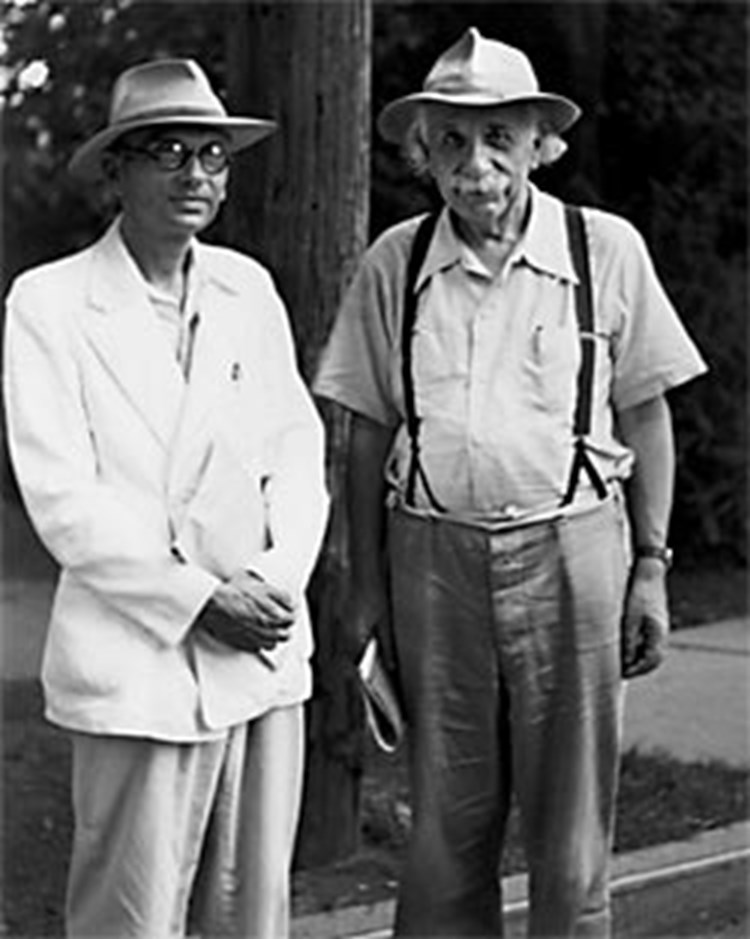
\includegraphics[width=0.5\textwidth]{img/godel_albert}
				\caption{Kurt Gödel and Albert Einstein}
			\end{figure}
		\end{column}	
	\end{columns}
	\begin{block}{Fun fact}
		Kurt Gödel and Albert Einstein good friends. Although the quite large age difference and different subjects. They used to take walks from and to institute where they were working in Princeton. It was also quite fortuitous that both spoke german.
	\end{block}
\end{frame}
\begin{frame}
	\frametitle{A quick reminder of Axioms}
	 \begin{Definition}[Axiom]
	 	Statements that are true without a formal proof of them. \\ For example:
	 	\[x = y \land y = z \implies x = z\]
	  	\begin{center}
	  		"It is possible to draw a straight line from any point to any other point"
	  	\end{center}
	 \end{Definition}
	 \begin{itemize}
	 	\item Any mathematical system starts out with a set of axioms
	 \end{itemize}
\end{frame}
\subsection{What is Completness?}
\begin{frame}
	\frametitle{Completness}
	 \begin{Definition}[Complete]
	 	A set of axioms is (syntactically, or negation-) complete if, for any statement in the axioms' language, that statement or its negation is provable from the axioms. \cite{smith}
	 \end{Definition}
\end{frame}
% first theorem
\section{First Incompletness Theorem}
\subsection{Overview}
\begin{frame}
	\frametitle{Gödel's First Incompletness Theorem}
	\begin{block}{The First Incompletness Theorem}
		If axioms do not contradict each other and are computably enumerable some statements are true, but cannot be proofed.
	\end{block}
	\begin{Definition}[Computably Enumerable Language]
	A recursively enumerable language is a formal language for which there exists a Turing machine which will enumerate all valid strings of the language.
	\end{Definition}
\end{frame}
\begin{frame}
\subsection{An Informal Approach}
	\frametitle{Gödel's First Incompletness Theorem}
	\begin{itemize}
		\item \textbf{The goal is to have a set of axioms that is powerful enough to proof everything in mathematics.}
		\item The status quo is that we have some axioms that are unproofable. Wouldn't it just make sense to add these axioms to our system, that we have a complete system?
		\item To answer this question we actually have to take a look at the Gödel numbering.
	\end{itemize}
\end{frame}
\begin{frame}
	\frametitle{Gödel Numbering}
	\begin{itemize}
		\item Gödel encoded every axiom with a unique natural number.
		\item He basically allowed mathematics to talk about itself.
		\item The so called "Gödelisierung" is not limited to axioms. You can encode every word $\omega$ in a language $L$.
		\item You can compare this to a modern computer, every text you type is encoded, for example in ASCII. In the end it comes even down to an encoding of $0$s and $1$s.
	\end{itemize}
	A short side statement: those numbers can be absolutely huge.
\end{frame}
\begin{frame}
	\frametitle{Gödel's First Incompletness Theorem}
	\begin{itemize}
		\item Now back to our first question.
		\item We encode now the statement "This statement cannot be proved from the axioms".
		\item Since we can work with numbers now, we can set up an equation.
		\item \textbf{Remember} An equation is \textbf{always} true or false, in mathematics.
	\end{itemize}
\end{frame}

\begin{frame}
	\frametitle{Gödel's First Incompletness Theorem}
	\begin{itemize}
		\item We start now by saying this statement is false. 
		\item This means that "This statement is provable from the axioms" is true, but a provable statement must be true.
		\item So now we have started with something which we assumed was false and now we have deduced that it was actually true. 
		\item We have got a contradiction.
	\end{itemize}
\end{frame}

\begin{frame}
	\frametitle{Gödel's First Incompletness Theorem}
	\begin{itemize}
		\item Since we are assuming that mathematics is consistent we cannot have contradictions.
		\item That means it cannot be false. 
		\item We now can conclude that it must be true, since an equation must always be true or false.
		\item Now we reinterpret what it says "This statement cannot be proved from the axioms". We have now a statement that cannot be proofed with the axioms of mathematics.
	\end{itemize}
\end{frame}

\begin{frame}
	\frametitle{Gödel's First Incompletness Theorem}
	\begin{itemize}
		\item This is now really \textbf{important}: Within a system of mathematics with certain axioms we found a true statement within there which cannot be proved true with that system. We have proofed by working outside the system and looking in. \label{important}
		\item Since it is true we can add that as an axiom. It is a true statement, so it will not make something which is consistent inconsistent.
	\end{itemize}
\end{frame}

\begin{frame}
	\frametitle{Gödel's First Incompletness Theorem}
	\begin{itemize}
		\item Now back to our question. "Wouldn't it just make sense to add these axioms to our system, that we have a complete system?"
		\item We have just shown that it would be possible to add new axioms to the system. On the other hand we end up adding endless new axioms to our system. We are stuck in an endless loop.
	\end{itemize}
\end{frame}

\subsection{A Modern Approach}
\begin{frame}
	\frametitle{A Modern Approach}
	\begin{itemize}
		\item Now we are getting more formal and take a look at modern proofs and approaches about the theorem.
	\end{itemize}
\end{frame}

\begin{frame}
	\frametitle{Parameters of the Proofs}
	All of the modern proofs of Gödel's theorem do have the following five parameters: \\ \vspace{0.5cm}
	\begin{enumerate}
		\item the choice of a specific basic formal system $T;$
		\item the choice of a universal computation model on some family U of objects of $T$, where by such a model $I$ mean any mathematically rigorous definition of the notion of a $c.e.$ \footnote[frame]{$c.e. \ldots $ computably enumerable} set of elements of $U$ (or of a computable function from $U$ to $U$);
	\end{enumerate}
\end{frame}

\begin{frame}
	\frametitle{Parameters of the Proofs}
	\begin{enumerate}
	\setcounter{enumi}{2}
		\item the choice of a Gödel numbering, that is, an encoding of the syntax of the theory $T$ by objects in $U;$
		\item a proof of the enumerability of the system $T$ (in the sense of the chosen computation model and the Gödel numbering);
		\item a presentation of an example of an expressible non-c.e. set (together with the proof of its expressibility and non-enumerability).
	\end{enumerate}
	\begin{flushright}
		\cite{bekl}
	\end{flushright}
\end{frame}

\begin{frame}
	\frametitle{Parameters of the Proofs - Examples}
	To prove Gödel’s theorem, various authors have considered the following computation models: \\
	\begin{enumerate}
		\item $c.e.$ sets as projections of primitive recursive relations (Gödel);
		\item the Herbrand–Gödel computable functions and partial recursive functions (Kleene);
		\item elementary formal systems (Smullyan);
		\item Turing machines;
		\item $\Sigma$-definable relations (Ershov) and others.
	\end{enumerate}
	\begin{flushright}
		\cite{bekl}
	\end{flushright}
\end{frame}

\begin{frame}
	\frametitle{Simplified Proofs}
	We note immediately that many authors of simplified proofs of Gödel's theorem neglect some of these points due to their intuitive clearness, using, as a rule, an informal concept of algorithm and some of the forms of the Church–Turing thesis. For example, the enumerability of the arithmetic PA is intuitively clear. At the same time, an "honest" proof of this statement needs programming in the framework of the chosen computation model, that is, significant technical work in general.
	\begin{flushright}
		\cite{bekl}
	\end{flushright}
\end{frame}

\subsection{Gödel's Proof}
\begin{frame}
	\frametitle{What did Gödel actually do?}
	\begin{itemize}
		\item Choosing the apparatus of primitive recursive functions, Gödel managed quite effectively with the problem.
		\item In our opinion there are still no complete proofs of Gödel’s theorem that are essentially simpler than his own proof.
	\end{itemize}
	\begin{flushright}
		\cite{bekl}
	\end{flushright}
\end{frame}

\begin{frame}
	\frametitle{Gödel's Plan}
	This proof is based on the technical notion of $representability$ of a $function$ in a theory $T$ and in the construction of an arithmetical formula asserting its own unprovability. The plan of Gödel's proof can be described as follows: \cite{bekl}
\end{frame}

\begin{frame}
	\frametitle{Gödel's Plan}
	\begin{enumerate}
		\item the proof of the fact that the proof predicate $Prf_T (x, y) $ for the theory $T$ is primitive recursive;
		\item the proof of the fact that every primitive recursive function is representable in $T$ , which implies the decidability in $T$ of the predicate $Prf_T (x, y);$
	\end{enumerate}
\end{frame}

\begin{frame}
	\frametitle{Gödel's Plan}
	\begin{enumerate}
	\setcounter{enumi}{2}
		\item the construction of a formula $\psi$ such that
		\[ T \vdash \psi \leftrightarrow \neg \operatorname{Pr}_{T}\left(\text{\underline{$^{\lceil} \psi^{\rceil}$}}\right) \]
		, where $Prf_T(x)$ stands for the provability formula $\exists y Prf_{T}(x, y)$, and where we
		use the representability in $T$ of the substitution function.
	\end{enumerate}
	The proof is completed with the following argument, which shows that if $T$ is $\omega$-consistent, then the formula $\psi$ is unprovable and irrefutable in $T$.
	\begin{flushright}
		\cite{bekl}
	\end{flushright}
\end{frame}

\begin{frame}
	\frametitle{Dive Deeper}
	If you are interested to see the complete proofs i would suggest to check out the following resources.
	\begin{itemize}
		\item Gödel incompleteness theorems and the limits of their applicability. I by L. D. Beklemishev. Pages 29 - 33. \cite{bekl}
		\item Or you can even take a look a the original paper of Kurt Gödel himself. \cite{godel}  
	\end{itemize}
\end{frame}

\section{Second Incompletness Theorem}
\subsection{Overview}
\begin{frame}
	\frametitle{Gödel's Second Incompletness Theorem}
	\begin{itemize}
		\item Now we are going to a look on the mostly overlooked second theorem of Kurt Gödel.
	\end{itemize}
\end{frame}

\subsection{Overview}
\begin{frame}
	\frametitle{Gödel's Second Incompletness Theorem}
	\begin{itemize}
		\item The first theorem asserts that there is a sentence which is neither provable nor refutable in the theory P under consideration.
	\end{itemize}
	\begin{block}{The Second Incompletness Theorem}
		The second theorem asserts that for this sentence one can take a formalization in P of the statement that the theory P itself is consistent.
	\end{block}

\end{frame}

\begin{frame}
	\frametitle{A not so Formal Explanation}
	\begin{itemize}
		\item A consistent math system cannot prove its own consistency.
		\item Can you remember the first informal proof? We proofed it outside the system of mathematics.
		\hyperlink{important}{\beamergotobutton{take a look again}}
	\end{itemize}
\end{frame}

\subsection{The foo Program}
\begin{frame}
	\frametitle{Gödel's Second Incompletness Theorem}
	\begin{itemize}
		\item We now try get an understanding of it with a very informal approach.
		\item For this we take the Halting problem into consideration.
		\item The Halting problem and the second incompletness theorem are similar.
		\item The first theorem says that: any sufficiently expressive math system must be either incomplete or \textbf{inconsistent}.
		\item In a consistent system we can prove at most one statement. 
		\item [] For example, if a cow can fly or not.
	\end{itemize}
\end{frame}

\begin{frame}
	\frametitle{What we are trying to do now}
	\begin{enumerate}
		\item Assume that mathematic system is consistent
		\item Create a program foo
		\item Analyze foo
		\item Find out that mathematics system is incomplete
	\end{enumerate}
\end{frame}

\begin{frame}[fragile]
	\frametitle{The Program foo}
	\begin{itemize}
		\item foo iterates over every mathematical proof.
	\end{itemize}
	\begin{center}
	  \begin{lstlisting}[frame=single]
function foo (M : program) {
  for each proof p {
    if (p proves M(M) LOOPS) 
      return;
    if (p proves M(M) HALTS)
      loop();
  }
}
   \end{lstlisting}
   	\end{center}
\end{frame}

\begin{frame}[fragile]
	\frametitle{The Program foo}
	\begin{itemize}
		\item What will now happen if we put foo into foo like this foo(foo)?
	\end{itemize}
	\begin{center}
	  \begin{lstlisting}[frame=single]
function foo (foo : program) {
  for each proof p {
    if (p proves foo(foo) LOOPS) 
      return;
    if (p proves foo(foo) HALTS)
      loop();
  }
}
   \end{lstlisting}
   	\end{center}
\end{frame}

\begin{frame}
	\frametitle{foo inside foo}
	\begin{itemize}
		\item The program now should loop or halt.
		\item We will now take a look on both possibilities. 
	\end{itemize}
\end{frame}

\begin{frame}[fragile]
	\frametitle{The Program Loops}
	\begin{itemize}
		\item If the program loops we end up here:
		\begin{center}
	  \begin{lstlisting}
    if (p proves foo(foo) LOOPS) 
      return;
   \end{lstlisting}
   	\end{center}
		\item so foo halts.
		\item If a program halts there is a proof that it does so (step through the program until it returns).
	\end{itemize}
\end{frame}

\begin{frame}[fragile]
	\frametitle{The Program Halts}
	\begin{itemize}
		\item If the program loops we end up here:
		\begin{center}
	  \begin{lstlisting}
    if (p proves foo(foo) HALTS)
      loop();
   \end{lstlisting}
   	\end{center}
		\item foo loops indefinitely.
		\item It is approved that the program loops (step through the program until it loops indefinitely).
	\end{itemize}
\end{frame}

\begin{frame}
	\frametitle{What does this mean now?}
	\begin{itemize}
		\item We have both proofs that the program halts and loops and this contradicts our assumption of consistency. Therefore neither can be true.
		\item We end up that we cannot prove within our system if foo(foo) loops or halts. Our system is therefore incomplete.
		\item But what does foo(foo) actually do? It loops over every possible math proof endlessly.
	\end{itemize}
\end{frame}

\subsection{The Proof}
\begin{frame}
	\frametitle{The Parameters of the Proof}
	\begin{enumerate}
		\item Recursive arithmetization of the syntax of the language of $T$.
		\item $\Sigma_1$-definability of the recursively enumerable predicates.
		\item Provability in $T$ of true $\Sigma_1$ sentences of the language of arithmetic.
		\item Diagonalization.
		\item Provability in $T$ of some of the properties of the $Provability$ predicate $Bew_T$.
	\end{enumerate}
	Please note that the first four parameters were also used for proofing the first theorem. The fifth one, which is actually harder to prove is the crucial step for the second and stronger theorem.
	\begin{flushright}
		\cite{bag}
	\end{flushright}
\end{frame}

\subsection{A formal proof}
\begin{frame}
	\frametitle{How to make a formal proof of this}
	\begin{itemize}
		\item For a short proof you could use the Zermelo-Fraenkel set theory. The proof was done by T.Jech in 1994.
	\end{itemize}
	
	\begin{Theorem}
		\[\text{If } ZF \text{ is consistent, then } ZF \nvdash CON(ZF)\]
	\end{Theorem}
	
		\begin{itemize}
		\item If you are interested in this proof, or some other versions take the following paper into consideration \cite{bag}.
	\end{itemize}
\end{frame}

% citations
\section{Outro}
\subsection{Conclusion}
\begin{frame}
	\frametitle{The Take Home Messages are}
	\begin{itemize}
		\item \textbf{First theorem:} Any sufficiently expressive math system must be either incomplete or inconsistent.
		\item \textbf{Second theorem:} A consistent math system cannot prove its own consistency.
		\item Gödel's second theorem placed in doubt the possibility of realizing the most important thesis of the so called \href{https://en.wikipedia.org/wiki/Hilbert\%27s_problems}{\textit{Hilbert programme}}. \cite{bekl}
	\end{itemize}
\end{frame}

\subsection{Useful Links}
\begin{frame}
	\frametitle{Further reading if you are interested}
	\begin{itemize}
		\item \url{https://plato.stanford.edu/entries/goedel-incompleteness/}
		\item \url{https://www.scientificamerican.com/article/what-is-goumldels-proof/}
		\item \url{https://www.researchgate.net/publication/286918416_On_the_philosophical_relevance_of_Godel's_incompleteness_theorems}
	\end{itemize}

\end{frame}
\begin{frame}{References}
    \bibliographystyle{ieeetr}
    \bibliography{bibfile}
\end{frame}
\end{document}
